\documentclass[12pt]{article}
\usepackage[brazil]{babel}
\usepackage{graphicx}
\usepackage{mathtools}
\usepackage{float} 
\usepackage{xcolor}


\usepackage{array}
\usepackage{booktabs}



% margenes
\usepackage[a4paper,left=2cm,right=2cm,top=2cm]{geometry}

%opening
\title{\textbf{Modelagem de Escoamentos Turbulentos. \\Lista de Exercícios No. 1}}

\author{Cristian Herledy López Lara}
\date{Maio 2025}

\begin{document}
	
\maketitle


\section*{Questão 1}

\textbf{\underline{Desenvolvimento}}

A lei de potência é uma expressão usada para representar o perfil de velocidade através de um canal. 

\begin{equation}
	\frac{\bar{u}}{U}  =  (1-\frac{r}{R})  ^\frac{1}{n}
\end{equation}

A figura a seguir mostra a curva de velocidade para n = 7 (o valor mais comumente usado para escoamento turbulento) e também outros valores, como 2 e 10, que representam os perfis para escoamento laminar e turbulento, respectivamente. Devido à difusividade da turbulência, a velocidade próxima às paredes cai mais rapidamente. Portanto, o perfil é mais plano à medida que $r \rightarrow  0$.

\begin{figure}[H]
	\centering
	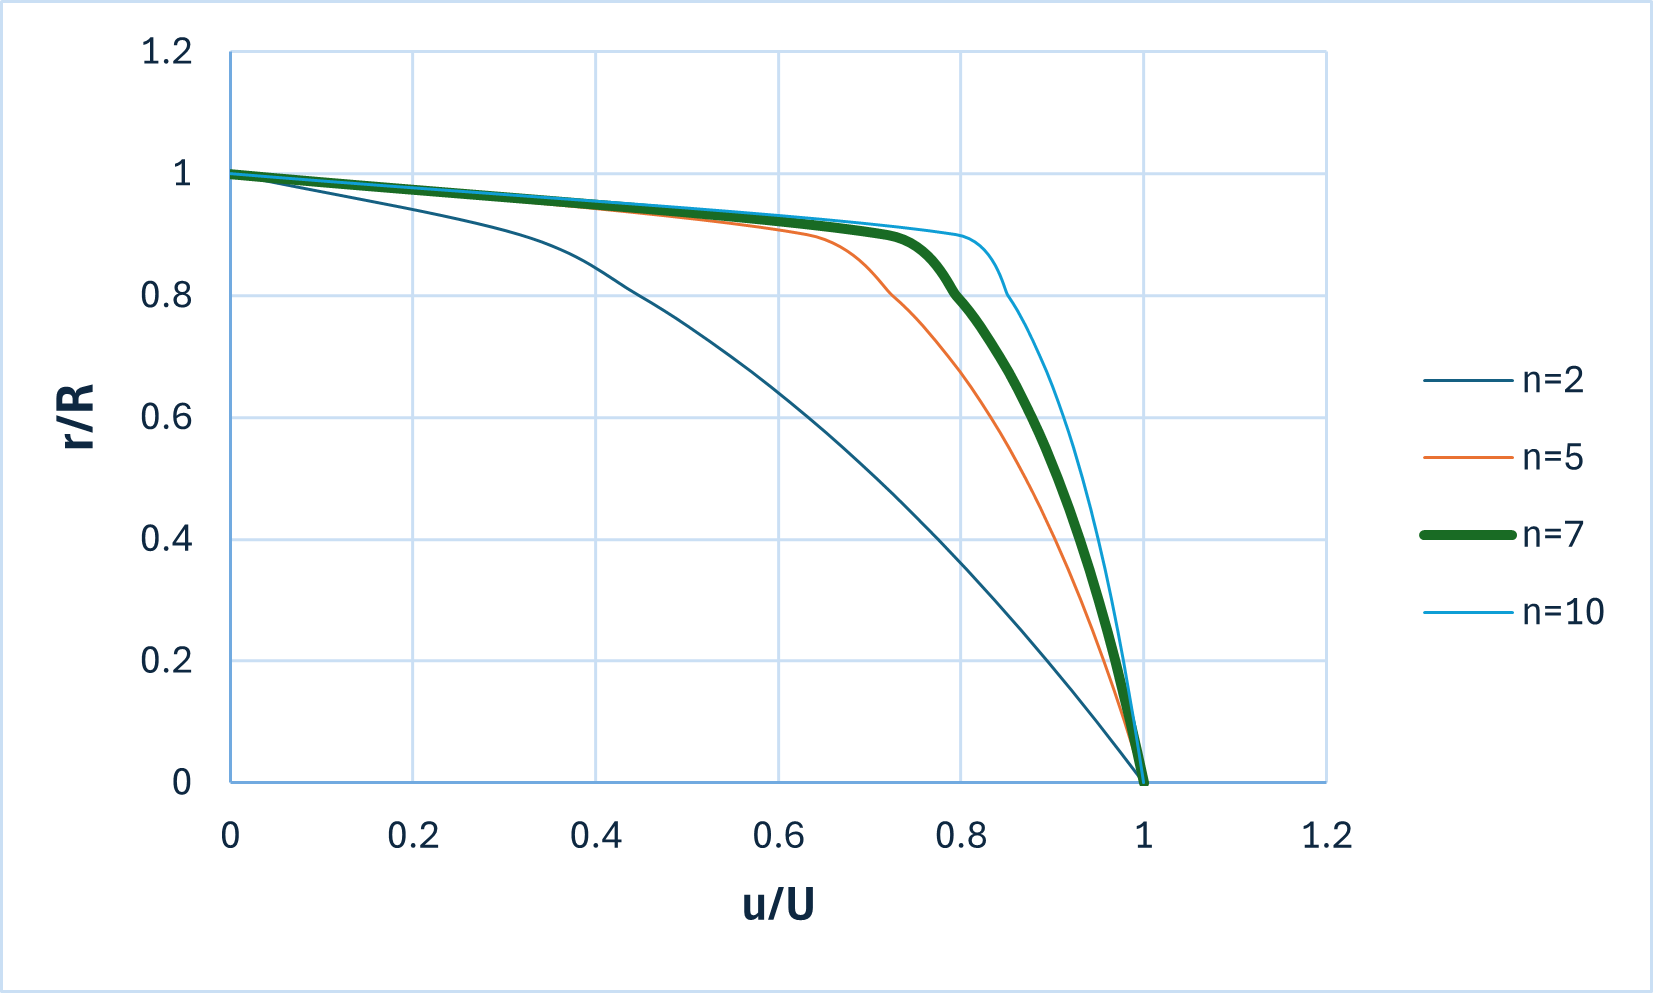
\includegraphics[width=.65\textwidth]{figures/1}
	\caption{Perfil de velocidade para escoamentos  0laminar y turbulento a traves da Lei de potencia}
\end{figure}

A expressão da lei de potência tem as seguintes inconsistências.

\subsection*{Inconsistência 1}

\begin{equation}
	\frac{\partial u}{\partial r}  =  -\frac{U}   {7(1-\frac{r}{R})  ^\frac{1}{7}}
\end{equation}

Quando $r = 0$, no eixo central de simetría da tubulação

\begin{equation}
	\frac{\partial u}{\partial r}  =  -\frac{U}   {7{}  ^\frac{1}{7}}
\end{equation}

A pendiente da curva é diferente de zero, Portanto, é inconsistente, visto que a velocidade no centro é máxima e sua derivada em relação a r deveria ser zero. Isso também sugere que a tensão de cisalhamento $\tau = \mu \frac{\partial u}{\partial r}$ neste ponto é negativa, que na realidade também deveria ser zero.

\subsection*{Inconsistência 2}

\begin{equation}
	\frac{\partial u}{\partial r}  =  -\frac{U}   {7(1-\frac{r}{R})  ^\frac{1}{7}}
\end{equation}

Quando $r = R$, na parede da tubulação
\begin{equation}
	\frac{\partial u}{\partial r}  =  -\frac{U}   {0{}  ^\frac{1}{7}} \sim -\infty
\end{equation}
Este valor na parede também é inconsistente, uma vez que o valor da tensão de cisalhamento $\tau = \mu \frac{\partial u}{\partial r} \rightarrow -\infty$, o que não é fisicamente possível, pois o escoamento seria completamente restrito.

\section*{Questão 2}

\textbf{\underline{Desenvolvimento}}

Executando operações algébricas para as expressões, obtemos

\underline{Laminar:}
\begin{equation}
	Nu_x= Re^\frac{1}{2}_x Pr^\frac{1}{3}	
\end{equation}

\begin{equation}
	Nu_x= \left( \frac{\rho U x}{\mu}\right)^\frac{1}{2}      \left( \frac{\mu Cp}{k}\right)^{\frac{1}{3}} \ = \ \frac{ \textcolor{blue}{\rho^\frac{1}{2}}  U^\frac{1}{2} x^\frac{1}{2}    Cp^\frac{1}{3}	}{ {\textcolor{red}{\mu^\frac{1}{6}}} k^\frac{1}{3}}
\end{equation}


\underline{Turbulento:}
\begin{equation}
	Nu_x= Re^\frac{4}{5}_x Pr^\frac{1}{3}	
\end{equation}

\begin{equation}
	Nu_x= \left( \frac{\rho Ux}{\mu}\right)^\frac{4}{5}      \left( \frac{\mu Cp}{k}\right)^{\frac{1}{3}} \ = \ \frac{\textcolor{blue}{\rho^\frac{4}{5} }  U^\frac{4}{5} x^\frac{4}{5}    Cp^\frac{1}{3}	}{ {\textcolor{red}{\mu^\frac{7}{15}}}  k^\frac{1}{3}}
\end{equation}

É notável que as diferenças estejam nos parâmetros de densidade e viscosidade.

\begin{figure}[H]
	\centering
	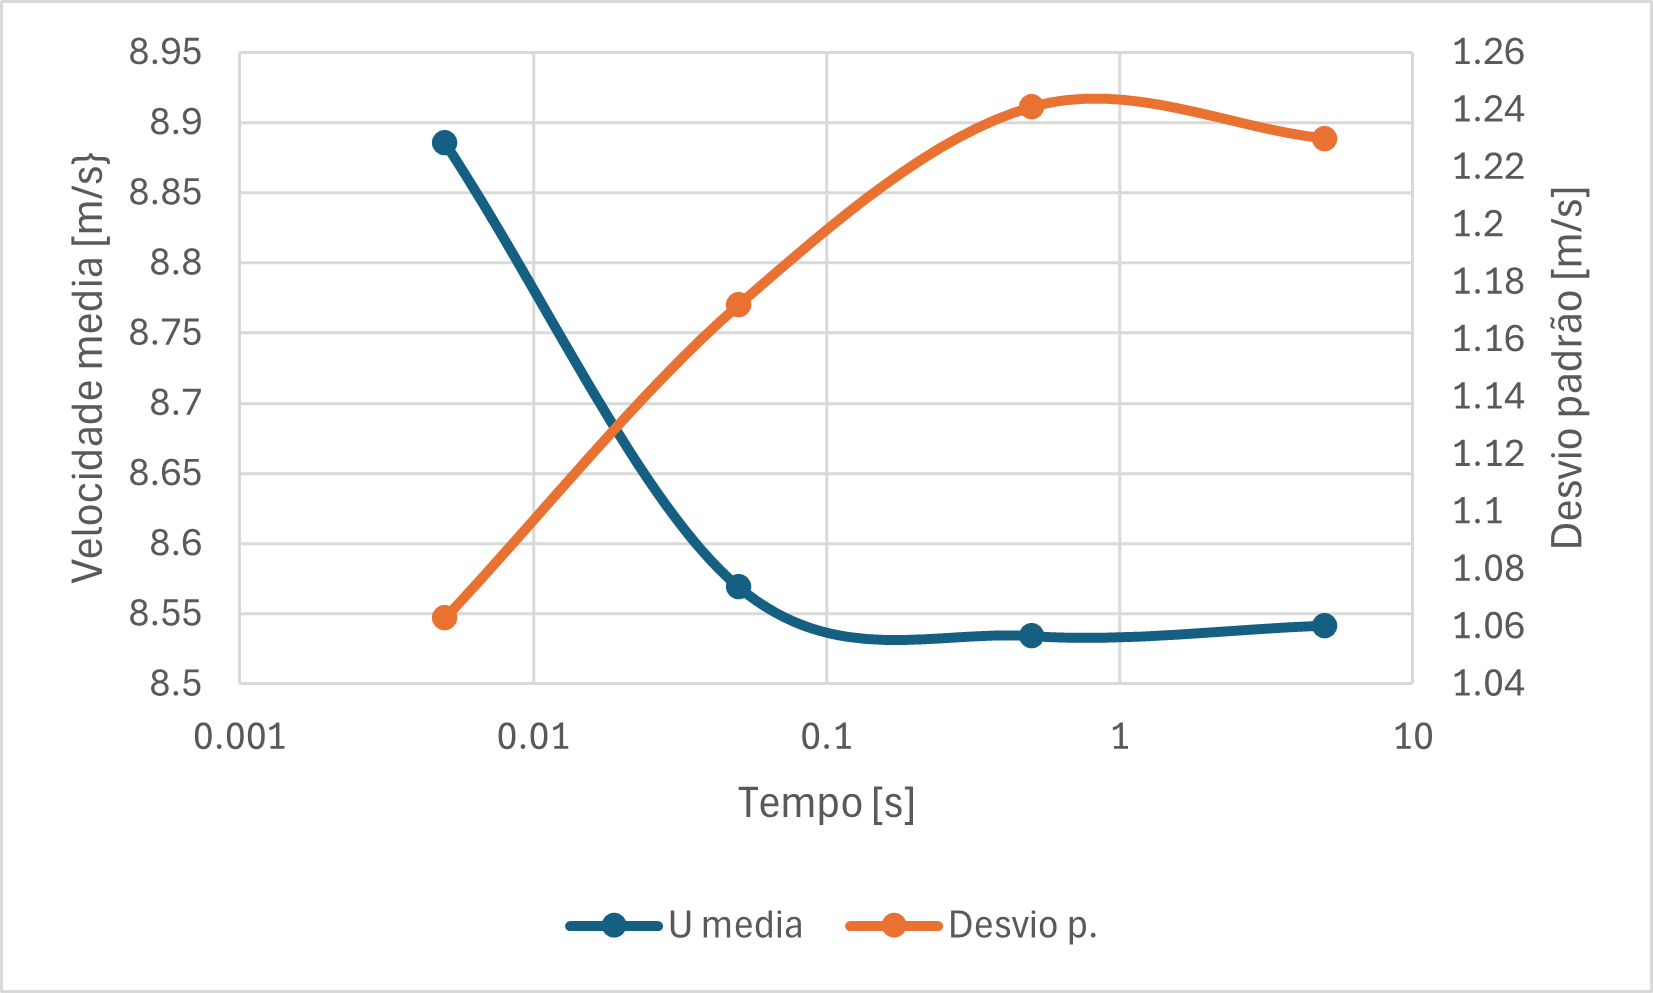
\includegraphics[width=.65\textwidth]{figures/2}
	\caption{Efeito da viscosidade em escoamentos laminar e turbulento}
\end{figure}

A viscosidade tem um efeito mais significativo no escoamento laminar. Isso ocorre porque, em problemas com números de Reynolds baixos, a troca de energia na forma de calor está associada ao fenômeno de difusão (o termo viscoso da equação de energia).

\begin{figure}[H]
	\centering
	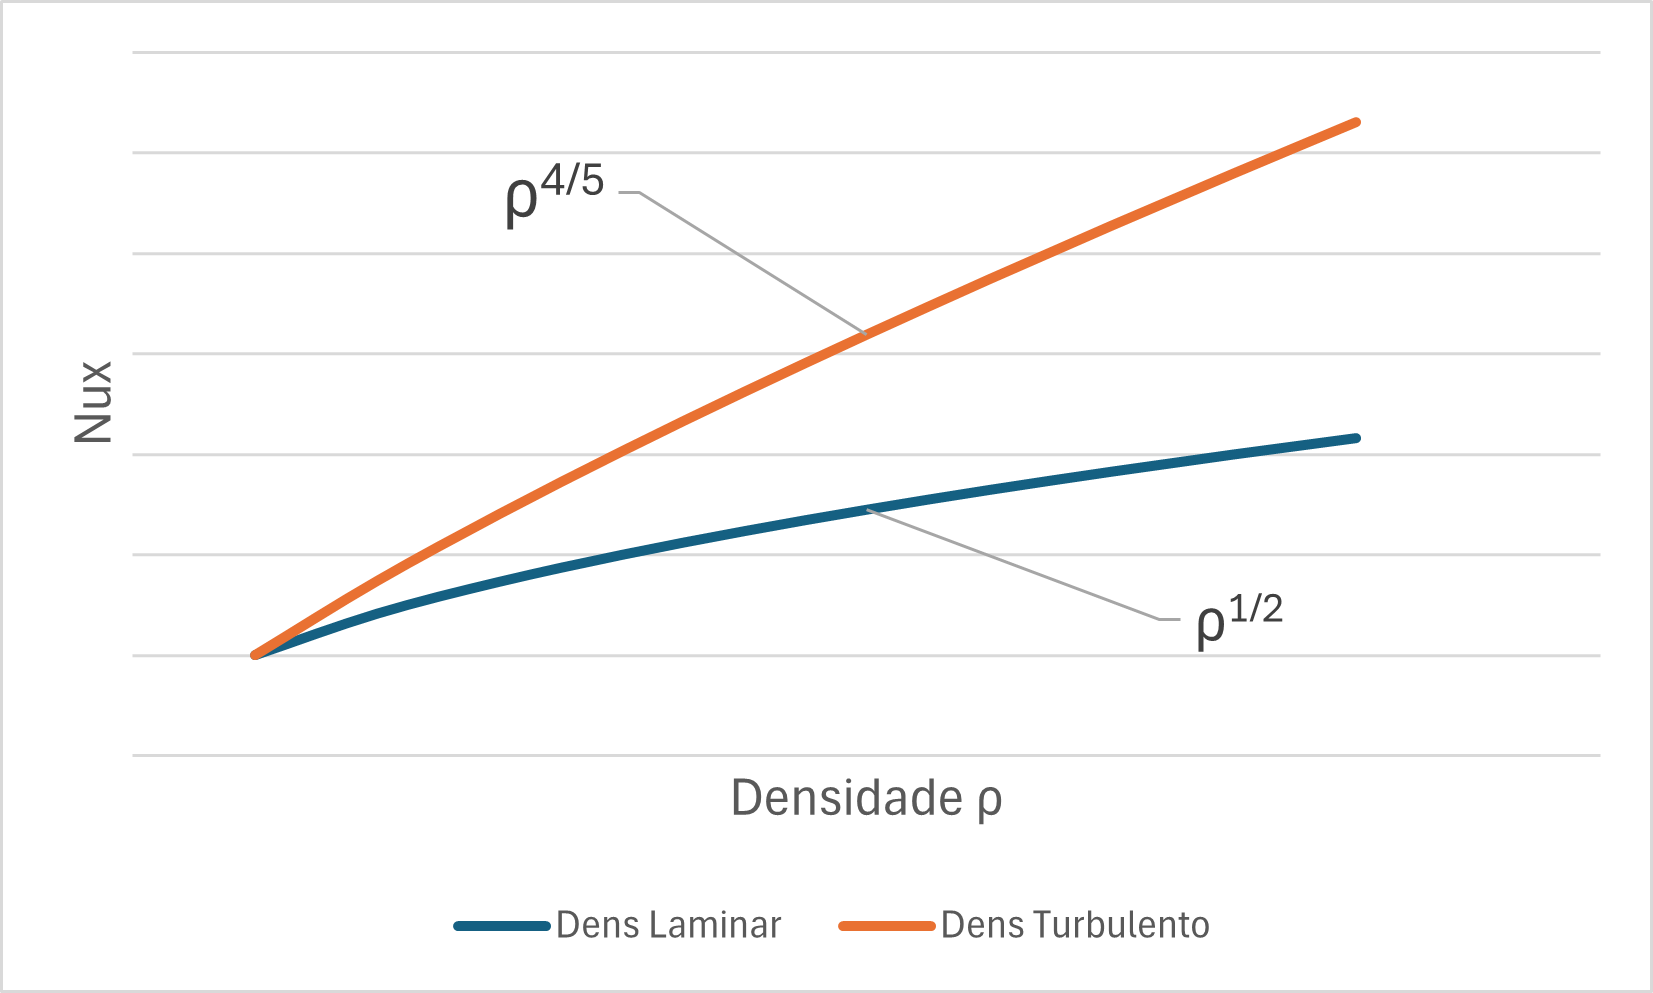
\includegraphics[width=.65\textwidth]{figures/3}
	\caption{Efeito da densidade em escoamentos laminar e turbulento}
\end{figure}


Por outro lado, a densidade é diretamente proporcional ao número de Nusselt (e ao coeficiente de transferência de calor). Isso se justifica considerando a física do fenômeno, visto que em escoamentos de alta velocidade a transferência de calor é realizada por advecção, o que tem um efeito direto na interação na escala das grandes estruturas do fluido.


\section*{Questão 3}

\textbf{\underline{Desenvolvimento}}


Partindo da expressão da equação de movimento na forma vetorial

\begin{equation}
	\frac{D\vec{u}}{Dt} = \frac{1}{\rho} \bigtriangledown p + \vec{f} \ + \nu \bigtriangledown^2 \vec{u}
\end{equation}


Desprezando as forças de campo e abrindo a derivada material


\begin{equation}
	\frac{\partial \vec{u}}{\partial t} + \vec{u} \cdot \bigtriangledown \vec{u} = \frac{1}{\rho} \bigtriangledown p + \nu \bigtriangledown^2 \vec{u}
\end{equation}


Da definicão de vorticidade que é dada pela expressão $\vec{\omega} = \bigtriangledown \otimes \vec{u}$, o rotacional é aplicado a equação de movimento

\begin{equation}
	\bigtriangledown \otimes \left( \frac{\partial \vec{u}}{\partial t} + \vec{u} \cdot \bigtriangledown \vec{u} = \frac{1}{\rho} \bigtriangledown p + \nu \bigtriangledown^2 \vec{u}\right) 
\end{equation}

\begin{equation}
	\bigtriangledown \otimes \frac{\partial \vec{u}}{\partial t} + \bigtriangledown \otimes \vec{u} \cdot \bigtriangledown \vec{u} = \bigtriangledown \otimes \frac{1}{\rho} \bigtriangledown p + \bigtriangledown \otimes \nu \bigtriangledown^2 \vec{u} 
\end{equation}

Usando a identidade $\vec{u} \cdot \bigtriangledown \vec{u} = (\bigtriangledown \otimes \vec{u}) \otimes \vec{u} + \frac{1}{2} \bigtriangledown(\vec{u}\cdot \vec{u})$



\begin{equation}
	\bigtriangledown \otimes \frac{\partial \vec{u}}{\partial t} + \bigtriangledown \otimes \left( \vec{\omega} \otimes \vec{u} + \frac{1}{2} \bigtriangledown(\vec{u}\cdot \vec{u})\right)   = \bigtriangledown \otimes \left( \frac{1}{\rho} \bigtriangledown p\right)  + \bigtriangledown \otimes \left( \nu \bigtriangledown^2 \vec{u} \right) 
\end{equation}

Como $\bigtriangledown \otimes \bigtriangledown f = 0$


\begin{equation}
	\bigtriangledown \otimes \frac{\partial \vec{u}}{\partial t} + \bigtriangledown \otimes \left( \vec{\omega} \otimes \vec{u} \right)   = \bigtriangledown \otimes \left( \nu \bigtriangledown^2 \vec{u} \right) 
\end{equation}

Com a identidade $\bigtriangledown \otimes \bigtriangledown^2 \vec{f} = \bigtriangledown^2(\bigtriangledown \otimes \vec{f})$

\begin{equation}
	\bigtriangledown \otimes \frac{\partial \vec{u}}{\partial t} + \bigtriangledown \otimes \left( \vec{\omega} \otimes \vec{u} \right)   = \nu\bigtriangledown^2 \left(  \bigtriangledown \otimes \vec{u} \right) 
\end{equation}

Usando a identidade $\bigtriangledown \otimes (\vec{\omega} \otimes \vec{u}) = (\vec{u} \cdot \bigtriangledown) \cdot \vec{\omega} - (\bigtriangledown \cdot \vec{\omega}) \vec{u} - (\vec{\omega}\cdot \bigtriangledown) \vec{u} + \vec{\omega}(\bigtriangledown \cdot \vec{u}) $

\begin{equation}
	\bigtriangledown \otimes \frac{\partial \vec{u}}{\partial t} + \left( (\vec{u} \cdot \bigtriangledown) \cdot \vec{\omega} - (\bigtriangledown \cdot \vec{\omega}) \vec{u} - (\vec{\omega}\cdot \bigtriangledown) \vec{u} + \vec{\omega}(\bigtriangledown \cdot \vec{u})\right)   = \nu\bigtriangledown^2 \left(  \bigtriangledown \otimes \vec{u} \right) 
\end{equation}

Considerando que $ \bigtriangledown \cdot \vec{f} = 0$

\begin{equation}
	\bigtriangledown \otimes \frac{\partial \vec{u}}{\partial t} + \left( (\vec{u} \cdot \bigtriangledown) \cdot \vec{\omega}  - (\vec{\omega}\cdot \bigtriangledown) \vec{u}\right)   = \nu\bigtriangledown^2 \left(  \bigtriangledown \otimes \vec{u} \right) 
\end{equation}

\begin{equation}
	\frac{\partial (\bigtriangledown \otimes \vec{u})}{\partial t} +  (\vec{u} \cdot \bigtriangledown) \cdot \vec{\omega}   = (\vec{\omega}\cdot \bigtriangledown) \vec{u} + \nu\bigtriangledown^2 \left(  \bigtriangledown \otimes \vec{u} \right) 
\end{equation}

\begin{equation}
	\frac{\partial \vec{\omega}}{\partial t} +  (\vec{u} \cdot \bigtriangledown) \cdot \vec{\omega}   = (\vec{\omega}\cdot \bigtriangledown) \vec{u} + \nu\bigtriangledown^2 \vec{\omega}
\end{equation}

Que na forma de notação indicial fica


\begin{equation}
	\frac{\partial \vec{\omega_i}}{\partial t} +  U_i \frac{\partial \vec{\omega}_i}{\partial x_j}= \vec{\omega_i}\ \frac{\partial \vec{U_i}}{\partial x_j} + \nu \frac{\partial^2 \vec{\omega_i}}{\partial x_j \partial x_i}
\end{equation}

Do termo da geraçao de vorticidade $\vec{\omega_i}\ \frac{\partial \vec{U_i}}{\partial x_j}$

\begin{equation}
	\vec{\omega} = \bigtriangledown \otimes \vec{u} \ = \ \left( \frac{\partial u_3}{\partial x_2} - \frac{\partial u_2}{\partial x_3}\right) \hat{e_1} - \left( \frac{\partial u_3}{\partial x_1} - \frac{\partial u_1}{\partial x_3}\right) \hat{e_2} + \left( \frac{\partial u_2}{\partial x_1} - \frac{\partial u_1}{\partial x_2}\right) \hat{e_3}
\end{equation}

Como em um escoamento 2D só temos as componentes $x_1 $ e $x_2$


\begin{equation}
	\vec{\omega} = \bigtriangledown \otimes \vec{u} \ = \ 0 \hat{e_1} - 0 \hat{e_2} + \left( \frac{\partial u_2}{\partial x_1} - \frac{\partial u_1}{\partial x_2}\right) \hat{e_3}
\end{equation}

A componente $\hat{e_3}$ é nula para o escoamento bidimensional.


\section*{Questão 4}

\textbf{\underline{Desenvolvimento}}

Partindo da expressão da equação de movimento de Cauchy na forma vetorial

\begin{equation}
	\rho \frac{D\vec{u}}{Dt} = \rho\vec{f} \ + \bigtriangledown \cdot \ \bar{\bar{T}} 
\end{equation}


E multiplicando por $\vec{u}$


\begin{equation}
	\vec{u}\rho \frac{D\vec{u}}{Dt} = \vec{u}\rho\vec{f} \ + \vec{u}\bigtriangledown \cdot \ \bar{\bar{T}} 
\end{equation}

Lembrando a definição de trabaloh total por unidade de volume


\begin{equation}
	\bigtriangledown \vec{u} \cdot \bar{\bar{T}} =  \bar{\bar{T}}  \bigtriangledown  \cdot \vec{u}  + \vec{u} \bigtriangledown  \cdot \bar{\bar{T}} 
\end{equation}

Onde o primeiro termo do lado dereito é equivalente a deformação por trabalho e o segundo é o incremento da energia cinêtica. Usando a simetria do tensor tensão, em notação indicial temos que ($e_{ij} = \bar{\bar{D}}$)

\begin{equation}
	 \bar{\bar{T}}  \bigtriangledown  \cdot \vec{u} =  \tau_{ij} \frac{\partial U_i}{\partial x_j} = \tau_{ij} e_{ij}
\end{equation}

Agora, com a definição do tensor tensão e sustituindo na eq. (27)

\begin{equation}
	\tau_{ij} =  -p\delta_{ij} + \frac{2}{3} \mu (\bigtriangledown \cdot \vec{u})\delta_{ij} + 2 \mu e_{ij}	
\end{equation}

\begin{equation}
	\tau_{ij} \frac{\partial U_i}{\partial x_j} = -p \bigtriangledown  \cdot \vec{u} - \frac{2}{3} \mu (\bigtriangledown \cdot \vec{u})^{2} + 2 \mu e_{ij}	e_{ij}
\end{equation}

Considerando que $e_{ij} = \frac{1}{2}\left( \frac{\partial U_i}{\partial x_j} + \frac{\partial U_j}{\partial x_i}\right) $ o termo de dissipação viscosa fica
\begin{equation}
	 2 \frac{\mu}{\rho} e_{ij}e_{ij} = \left( \frac{1}{2}\left( \frac{\partial U_i}{\partial x_j} + \frac{\partial U_j}{\partial x_i}\right)  \frac{1}{2}\left( \frac{\partial U_i}{\partial x_j} + \frac{\partial U_j}{\partial x_i}\right)  \right) 
\end{equation}
\begin{equation}
	2 \frac{\mu}{\rho} e_{ij}e_{ij} = \frac{2}{4} \nu\left( \left( \frac{\partial U_i}{\partial x_j} + \frac{\partial U_j}{\partial x_i}\right)  \left( \frac{\partial U_i}{\partial x_j} + \frac{\partial U_j}{\partial x_i}\right)  \right) 
\end{equation}

\begin{equation}
	\bigtriangleup = \frac{1}{2} \nu\left( \left( \frac{\partial U_i}{\partial x_j} + \frac{\partial U_j}{\partial x_i}\right)  \left( \frac{\partial U_i}{\partial x_j} + \frac{\partial U_j}{\partial x_i}\right)  \right) 
\end{equation}


\section*{Questão 4}

\textbf{\underline{Desenvolvimento}}

\begin{figure}[H]
	\centering
	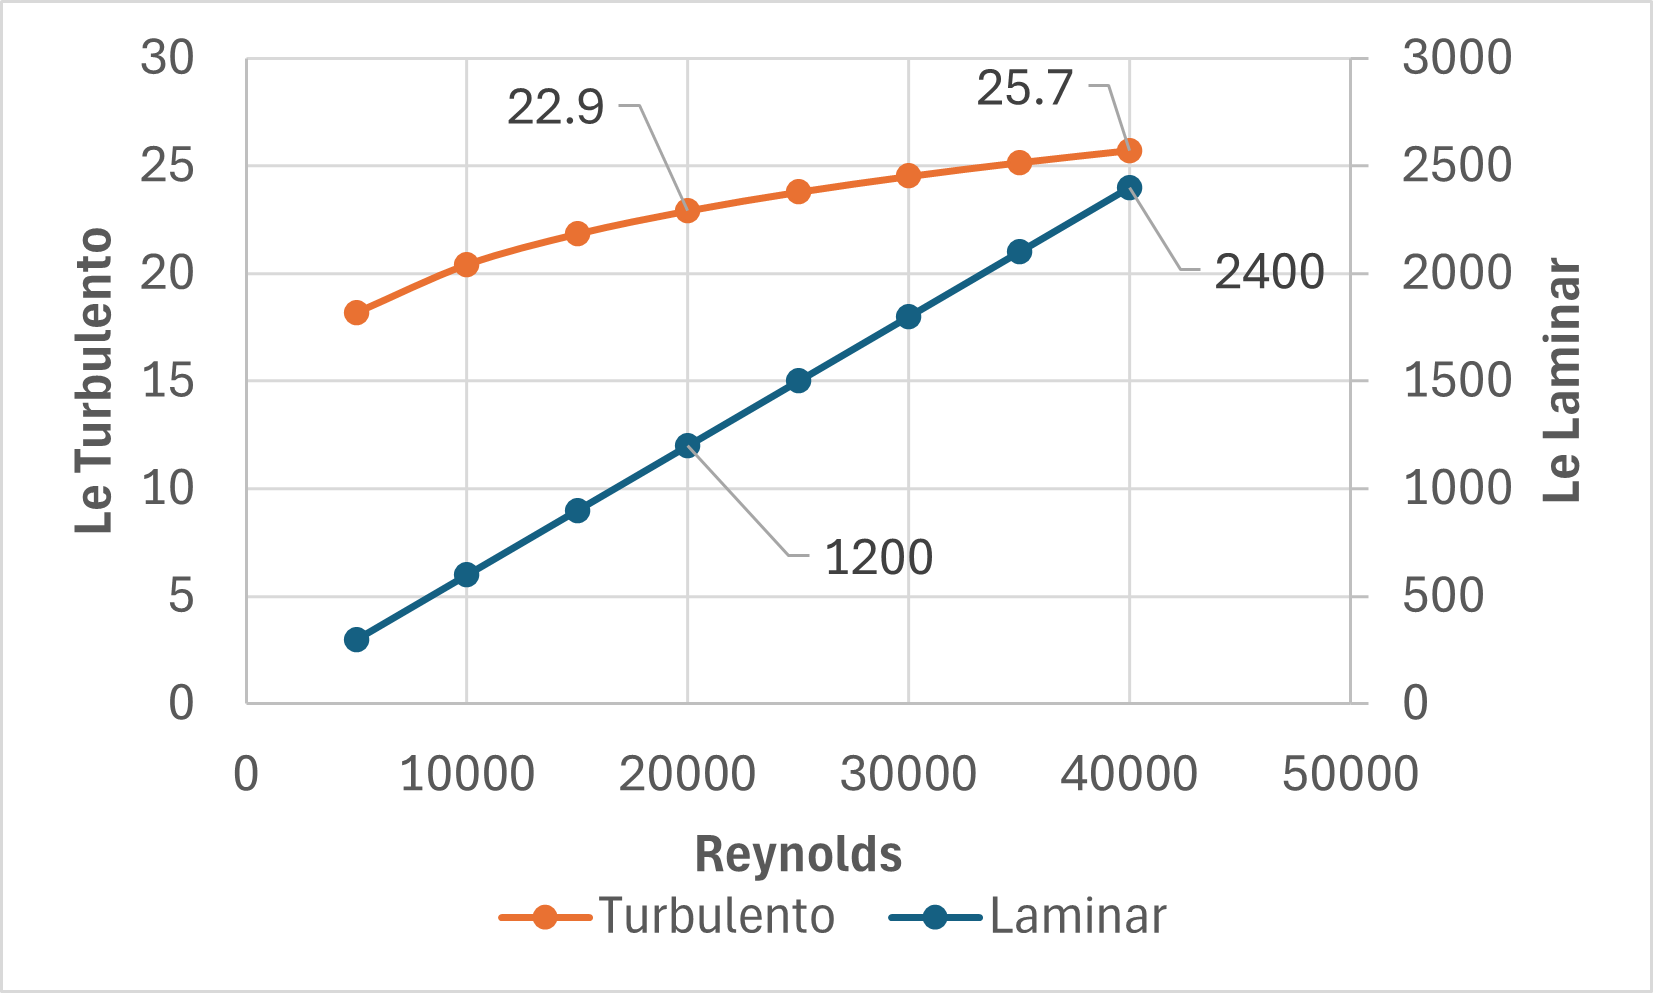
\includegraphics[width=.65\textwidth]{figures/4}
	\caption{Evolução da Le como função do numero de Reynols em regimes laminar e turbulento}
\end{figure}

O gráfico acima foi construído com as expressões da Lista, para observar a evolução dos valores do comprimento de entrada $L_e$ em relação ao aumento do número de Reynolds para escoamentos laminares e turbulentos (o diâmetro é o mesmo em ambos os casos). 

O comprimento de entrada é significativamente maior no regime laminar do que no regime turbulento, e isso é justificado pela presença de estruturas de pequena e grande escala no escoamento turbulento, o que torna o transporte de momento muito mais eficiente e o escoamento se desenvolve mais rapidamente.

Para um número de Reynolds de 40.000, o comprimento de entrada para escoamento laminar aumenta em 100\%, enquanto para escoamento turbulento aumenta em 11\%. Conclui-se que, em números de Reynolds altos, o escoamento totalmente desenvolvido é alcançado com comprimentos de entrada muito menores.

\begin{thebibliography}{999}
	
	
	\bibitem{Kundu}
	Pijush Kundu,
	Fluid Mechanics.
	San Diego, California USA,
	2nd Edition,
	2004.
	
	\bibitem{Prata}
	Alvaro Prata,
	Fundamentos da mecanica dos fluidos.
	Florianopolis UFSC, Brasil,
	1ra edição,
	2023.
	
	
\end{thebibliography}


\end{document}





